\documentclass[twoside]{book}

% Packages required by doxygen
\usepackage{fixltx2e}
\usepackage{calc}
\usepackage{doxygen}
\usepackage[export]{adjustbox} % also loads graphicx
\usepackage{graphicx}
\usepackage[utf8]{inputenc}
\usepackage{makeidx}
\usepackage{multicol}
\usepackage{multirow}
\PassOptionsToPackage{warn}{textcomp}
\usepackage{textcomp}
\usepackage[nointegrals]{wasysym}
\usepackage[table]{xcolor}

% Font selection
\usepackage[T1]{fontenc}
\usepackage[scaled=.90]{helvet}
\usepackage{courier}
\usepackage{amssymb}
\usepackage{sectsty}
\renewcommand{\familydefault}{\sfdefault}
\allsectionsfont{%
  \fontseries{bc}\selectfont%
  \color{darkgray}%
}
\renewcommand{\DoxyLabelFont}{%
  \fontseries{bc}\selectfont%
  \color{darkgray}%
}
\newcommand{\+}{\discretionary{\mbox{\scriptsize$\hookleftarrow$}}{}{}}

% Page & text layout
\usepackage{geometry}
\geometry{%
  a4paper,%
  top=2.5cm,%
  bottom=2.5cm,%
  left=2.5cm,%
  right=2.5cm%
}
\tolerance=750
\hfuzz=15pt
\hbadness=750
\setlength{\emergencystretch}{15pt}
\setlength{\parindent}{0cm}
\setlength{\parskip}{3ex plus 2ex minus 2ex}
\makeatletter
\renewcommand{\paragraph}{%
  \@startsection{paragraph}{4}{0ex}{-1.0ex}{1.0ex}{%
    \normalfont\normalsize\bfseries\SS@parafont%
  }%
}
\renewcommand{\subparagraph}{%
  \@startsection{subparagraph}{5}{0ex}{-1.0ex}{1.0ex}{%
    \normalfont\normalsize\bfseries\SS@subparafont%
  }%
}
\makeatother

% Headers & footers
\usepackage{fancyhdr}
\pagestyle{fancyplain}
\fancyhead[LE]{\fancyplain{}{\bfseries\thepage}}
\fancyhead[CE]{\fancyplain{}{}}
\fancyhead[RE]{\fancyplain{}{\bfseries\leftmark}}
\fancyhead[LO]{\fancyplain{}{\bfseries\rightmark}}
\fancyhead[CO]{\fancyplain{}{}}
\fancyhead[RO]{\fancyplain{}{\bfseries\thepage}}
\fancyfoot[LE]{\fancyplain{}{}}
\fancyfoot[CE]{\fancyplain{}{}}
\fancyfoot[RE]{\fancyplain{}{\bfseries\scriptsize Generated by Doxygen }}
\fancyfoot[LO]{\fancyplain{}{\bfseries\scriptsize Generated by Doxygen }}
\fancyfoot[CO]{\fancyplain{}{}}
\fancyfoot[RO]{\fancyplain{}{}}
\renewcommand{\footrulewidth}{0.4pt}
\renewcommand{\chaptermark}[1]{%
  \markboth{#1}{}%
}
\renewcommand{\sectionmark}[1]{%
  \markright{\thesection\ #1}%
}

% Indices & bibliography
\usepackage{natbib}
\usepackage[titles]{tocloft}
\setcounter{tocdepth}{3}
\setcounter{secnumdepth}{5}
\makeindex

% Hyperlinks (required, but should be loaded last)
\usepackage{ifpdf}
\ifpdf
  \usepackage[pdftex,pagebackref=true]{hyperref}
\else
  \usepackage[ps2pdf,pagebackref=true]{hyperref}
\fi
\hypersetup{%
  colorlinks=true,%
  linkcolor=blue,%
  citecolor=blue,%
  unicode%
}

% Custom commands
\newcommand{\clearemptydoublepage}{%
  \newpage{\pagestyle{empty}\cleardoublepage}%
}

\usepackage{caption}
\captionsetup{labelsep=space,justification=centering,font={bf},singlelinecheck=off,skip=4pt,position=top}

%===== C O N T E N T S =====

\begin{document}

% Titlepage & ToC
\hypersetup{pageanchor=false,
             bookmarksnumbered=true,
             pdfencoding=unicode
            }
\pagenumbering{alph}
\begin{titlepage}
\vspace*{7cm}
\begin{center}%
{\Large Doxygen Testing }\\
\vspace*{1cm}
{\large Generated by Doxygen 1.8.13}\\
\end{center}
\end{titlepage}
\clearemptydoublepage
\pagenumbering{roman}
\tableofcontents
\clearemptydoublepage
\pagenumbering{arabic}
\hypersetup{pageanchor=true}

%--- Begin generated contents ---
\chapter{R\+E\+A\+D\+ME}
\label{md_README}
\Hypertarget{md_README}
\#\+Employees-\/\+Management 
\chapter{Hierarchical Index}
\section{Class Hierarchy}
This inheritance list is sorted roughly, but not completely, alphabetically\+:\begin{DoxyCompactList}
\item \contentsline{section}{Employee}{\pageref{classEmployee}}{}
\begin{DoxyCompactList}
\item \contentsline{section}{Officer}{\pageref{classOfficer}}{}
\item \contentsline{section}{Supervisor}{\pageref{classSupervisor}}{}
\end{DoxyCompactList}
\end{DoxyCompactList}

\chapter{Class Index}
\section{Class List}
Here are the classes, structs, unions and interfaces with brief descriptions\+:\begin{DoxyCompactList}
\item\contentsline{section}{\hyperlink{classEmployee}{Employee} }{\pageref{classEmployee}}{}
\item\contentsline{section}{\hyperlink{classOfficer}{Officer} }{\pageref{classOfficer}}{}
\item\contentsline{section}{\hyperlink{classSupervisor}{Supervisor} }{\pageref{classSupervisor}}{}
\end{DoxyCompactList}

\chapter{File Index}
\section{File List}
Here is a list of all documented files with brief descriptions\+:\begin{DoxyCompactList}
\item\contentsline{section}{\hyperlink{Employee_8cpp}{Employee.\+cpp} \\*Class implementation }{\pageref{Employee_8cpp}}{}
\item\contentsline{section}{\hyperlink{Employee_8h}{Employee.\+h} \\*Class defintions for the \hyperlink{classEmployee}{Employee} class }{\pageref{Employee_8h}}{}
\item\contentsline{section}{\hyperlink{main_8cpp}{main.\+cpp} \\*Main }{\pageref{main_8cpp}}{}
\item\contentsline{section}{\hyperlink{Officer_8cpp}{Officer.\+cpp} \\*\hyperlink{classOfficer}{Officer} class implementation }{\pageref{Officer_8cpp}}{}
\item\contentsline{section}{{\bfseries Officer.\+h} }{\pageref{Officer_8h}}{}
\item\contentsline{section}{\hyperlink{Supervisor_8cpp}{Supervisor.\+cpp} \\*\hyperlink{classSupervisor}{Supervisor} implementatiom }{\pageref{Supervisor_8cpp}}{}
\item\contentsline{section}{\hyperlink{Supervisor_8h}{Supervisor.\+h} \\*\hyperlink{classSupervisor}{Supervisor} class implementation }{\pageref{Supervisor_8h}}{}
\end{DoxyCompactList}

\chapter{Class Documentation}
\hypertarget{classEmployee}{}\section{Employee Class Reference}
\label{classEmployee}\index{Employee@{Employee}}


Inheritance diagram for Employee\+:\nopagebreak
\begin{figure}[H]
\begin{center}
\leavevmode
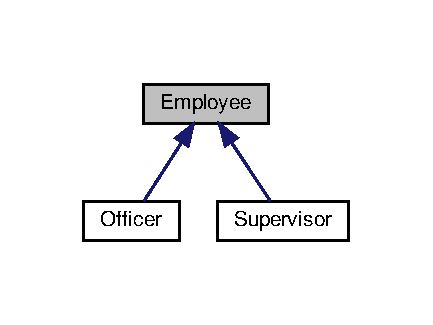
\includegraphics[width=208pt]{classEmployee__inherit__graph}
\end{center}
\end{figure}
\subsection*{Public Member Functions}
\begin{DoxyCompactItemize}
\item 
\mbox{\Hypertarget{classEmployee_a79556ad700627dba88049f487a34a762}\label{classEmployee_a79556ad700627dba88049f487a34a762}} 
virtual void {\bfseries print} ()
\item 
\mbox{\Hypertarget{classEmployee_a01c2c44e15434237db28832f6972e960}\label{classEmployee_a01c2c44e15434237db28832f6972e960}} 
virtual double {\bfseries calculate\+Pay} ()
\item 
\mbox{\Hypertarget{classEmployee_a67c345031cf63f515fb09dc675dee5f3}\label{classEmployee_a67c345031cf63f515fb09dc675dee5f3}} 
void {\bfseries anniversary} ()
\item 
\mbox{\Hypertarget{classEmployee_ad0c935ef9a290a82dcf7865172c90148}\label{classEmployee_ad0c935ef9a290a82dcf7865172c90148}} 
{\bfseries Employee} (int ID, int years, double hourly\+Rate, float hours\+Worked)
\end{DoxyCompactItemize}
\subsection*{Protected Attributes}
\begin{DoxyCompactItemize}
\item 
\mbox{\Hypertarget{classEmployee_ac31134abb9b4004fc015e51ef579b069}\label{classEmployee_ac31134abb9b4004fc015e51ef579b069}} 
double {\bfseries hourly\+Rate}
\item 
\mbox{\Hypertarget{classEmployee_afde35c73d02eb1cfe89e23a80998b42e}\label{classEmployee_afde35c73d02eb1cfe89e23a80998b42e}} 
float {\bfseries hours\+Worked}
\end{DoxyCompactItemize}
\subsection*{Private Attributes}
\begin{DoxyCompactItemize}
\item 
\mbox{\Hypertarget{classEmployee_a832bbae4ee8a704b917f82c4d497bbac}\label{classEmployee_a832bbae4ee8a704b917f82c4d497bbac}} 
int {\bfseries ID}
\item 
\mbox{\Hypertarget{classEmployee_a3e4862d9dfc73becb459a562fa2e25f5}\label{classEmployee_a3e4862d9dfc73becb459a562fa2e25f5}} 
int {\bfseries years}
\end{DoxyCompactItemize}


The documentation for this class was generated from the following files\+:\begin{DoxyCompactItemize}
\item 
Employee.\+h\item 
Employee.\+cpp\end{DoxyCompactItemize}

\hypertarget{classOfficer}{}\section{Officer Class Reference}
\label{classOfficer}\index{Officer@{Officer}}


Inheritance diagram for Officer\+:
\nopagebreak
\begin{figure}[H]
\begin{center}
\leavevmode
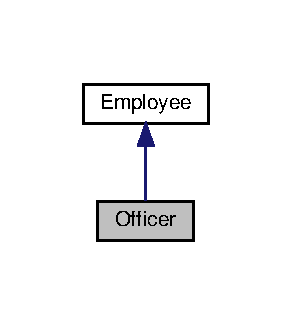
\includegraphics[width=140pt]{classOfficer__inherit__graph}
\end{center}
\end{figure}


Collaboration diagram for Officer\+:
\nopagebreak
\begin{figure}[H]
\begin{center}
\leavevmode
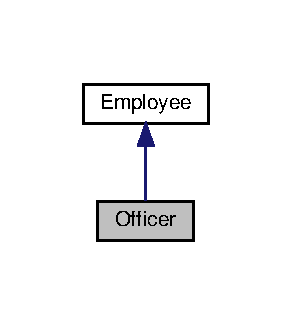
\includegraphics[width=140pt]{classOfficer__coll__graph}
\end{center}
\end{figure}
\subsection*{Public Member Functions}
\begin{DoxyCompactItemize}
\item 
\mbox{\Hypertarget{classOfficer_aeadece05a1a0b7fb29bd412830d2e07a}\label{classOfficer_aeadece05a1a0b7fb29bd412830d2e07a}} 
void {\bfseries print} ()
\item 
\mbox{\Hypertarget{classOfficer_a1fa1aad39b9e95be7a088990ebf17059}\label{classOfficer_a1fa1aad39b9e95be7a088990ebf17059}} 
double {\bfseries calculate\+Pay} ()
\item 
\mbox{\Hypertarget{classOfficer_ac75c45d6e8628606278cb4ce6596f67f}\label{classOfficer_ac75c45d6e8628606278cb4ce6596f67f}} 
{\bfseries Officer} (int ID, int years, double hourly\+Rate, float hours\+Worked, double evilness)
\end{DoxyCompactItemize}
\subsection*{Additional Inherited Members}


The documentation for this class was generated from the following files\+:\begin{DoxyCompactItemize}
\item 
Officer.\+h\item 
Officer.\+cpp\end{DoxyCompactItemize}

\hypertarget{classSupervisor}{}\section{Supervisor Class Reference}
\label{classSupervisor}\index{Supervisor@{Supervisor}}


Inheritance diagram for Supervisor\+:
\nopagebreak
\begin{figure}[H]
\begin{center}
\leavevmode
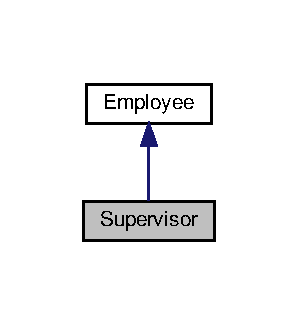
\includegraphics[width=143pt]{classSupervisor__inherit__graph}
\end{center}
\end{figure}


Collaboration diagram for Supervisor\+:
\nopagebreak
\begin{figure}[H]
\begin{center}
\leavevmode
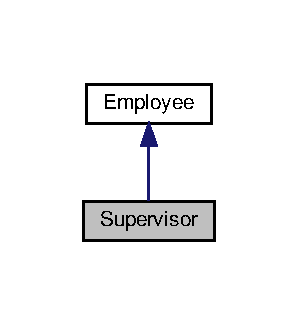
\includegraphics[width=143pt]{classSupervisor__coll__graph}
\end{center}
\end{figure}
\subsection*{Public Member Functions}
\begin{DoxyCompactItemize}
\item 
\mbox{\Hypertarget{classSupervisor_a92483dc9a54904d79b46c6ec4efb3f54}\label{classSupervisor_a92483dc9a54904d79b46c6ec4efb3f54}} 
void {\bfseries print} ()
\item 
\mbox{\Hypertarget{classSupervisor_aa37daa89523c08b84ae8141299e036f8}\label{classSupervisor_aa37daa89523c08b84ae8141299e036f8}} 
double {\bfseries calculate\+Pay} ()
\item 
\mbox{\Hypertarget{classSupervisor_a02d9245744652deb20e9408001d6ed3b}\label{classSupervisor_a02d9245744652deb20e9408001d6ed3b}} 
{\bfseries Supervisor} (int ID, int years, double hourly\+Rate, float hours\+Worked, int num\+Supervised)
\end{DoxyCompactItemize}
\subsection*{Additional Inherited Members}


The documentation for this class was generated from the following files\+:\begin{DoxyCompactItemize}
\item 
Supervisor.\+h\item 
Supervisor.\+cpp\end{DoxyCompactItemize}

\chapter{File Documentation}
\hypertarget{Employee_8cpp}{}\section{Employee.\+cpp File Reference}
\label{Employee_8cpp}\index{Employee.\+cpp@{Employee.\+cpp}}


Class implementation.  


{\ttfamily \#include \char`\"{}Employee.\+h\char`\"{}}\newline
{\ttfamily \#include $<$iostream$>$}\newline
Include dependency graph for Employee.\+cpp\+:
\nopagebreak
\begin{figure}[H]
\begin{center}
\leavevmode
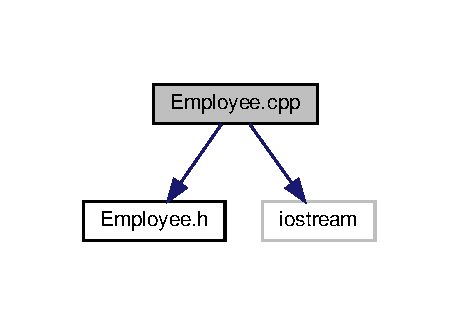
\includegraphics[width=220pt]{Employee_8cpp__incl}
\end{center}
\end{figure}


\subsection{Detailed Description}
Class implementation. 

\begin{DoxyAuthor}{Author}
Ethan Buchanan 
\end{DoxyAuthor}
\begin{DoxyDate}{Date}
2022-\/11-\/15 Implementation for employee class 
\end{DoxyDate}

\hypertarget{Employee_8h}{}\section{Employee.\+h File Reference}
\label{Employee_8h}\index{Employee.\+h@{Employee.\+h}}


Class defintions for the \hyperlink{classEmployee}{Employee} class.  


This graph shows which files directly or indirectly include this file\+:
\nopagebreak
\begin{figure}[H]
\begin{center}
\leavevmode
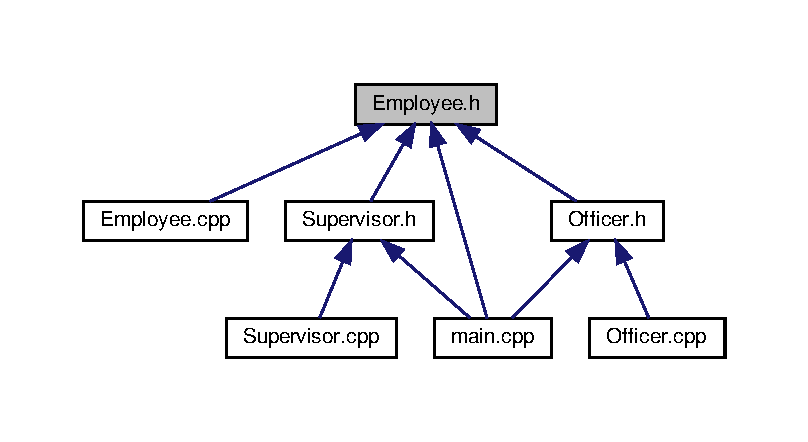
\includegraphics[width=350pt]{Employee_8h__dep__incl}
\end{center}
\end{figure}
\subsection*{Classes}
\begin{DoxyCompactItemize}
\item 
class \hyperlink{classEmployee}{Employee}
\end{DoxyCompactItemize}


\subsection{Detailed Description}
Class defintions for the \hyperlink{classEmployee}{Employee} class. 

\begin{DoxyAuthor}{Author}
Ethan Buchanan 
\end{DoxyAuthor}
\begin{DoxyDate}{Date}
2022-\/11-\/15 \hyperlink{classEmployee}{Employee} class definitions all you need to know 
\end{DoxyDate}

\hypertarget{main_8cpp}{}\section{main.\+cpp File Reference}
\label{main_8cpp}\index{main.\+cpp@{main.\+cpp}}


Main.  


{\ttfamily \#include $<$iostream$>$}\newline
{\ttfamily \#include \char`\"{}Employee.\+h\char`\"{}}\newline
{\ttfamily \#include \char`\"{}Supervisor.\+h\char`\"{}}\newline
{\ttfamily \#include \char`\"{}Officer.\+h\char`\"{}}\newline
Include dependency graph for main.\+cpp\+:\nopagebreak
\begin{figure}[H]
\begin{center}
\leavevmode
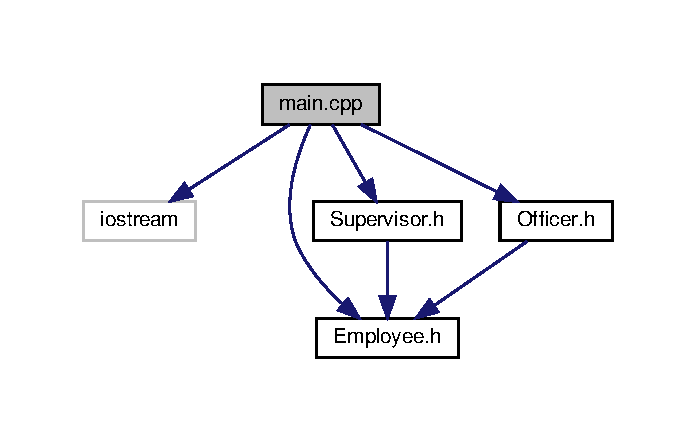
\includegraphics[width=334pt]{main_8cpp__incl}
\end{center}
\end{figure}
\subsection*{Functions}
\begin{DoxyCompactItemize}
\item 
\mbox{\Hypertarget{main_8cpp_a9ccea1912d6e2275d5612e294919d113}\label{main_8cpp_a9ccea1912d6e2275d5612e294919d113}} 
void {\bfseries run\+Employee\+Tests} (\hyperlink{classEmployee}{Employee} \&e)
\item 
\mbox{\Hypertarget{main_8cpp_ae66f6b31b5ad750f1fe042a706a4e3d4}\label{main_8cpp_ae66f6b31b5ad750f1fe042a706a4e3d4}} 
int {\bfseries main} ()
\end{DoxyCompactItemize}


\subsection{Detailed Description}
Main. 

\begin{DoxyAuthor}{Author}
Ethan Buchanan 
\end{DoxyAuthor}
\begin{DoxyDate}{Date}
2022-\/11-\/15 Prints and test the \hyperlink{classEmployee}{Employee} class and it derived classes 
\end{DoxyDate}

\hypertarget{Officer_8cpp}{}\section{Officer.\+cpp File Reference}
\label{Officer_8cpp}\index{Officer.\+cpp@{Officer.\+cpp}}


\hyperlink{classOfficer}{Officer} class implementation.  


{\ttfamily \#include \char`\"{}Officer.\+h\char`\"{}}\newline
{\ttfamily \#include $<$iostream$>$}\newline
Include dependency graph for Officer.\+cpp\+:
\nopagebreak
\begin{figure}[H]
\begin{center}
\leavevmode
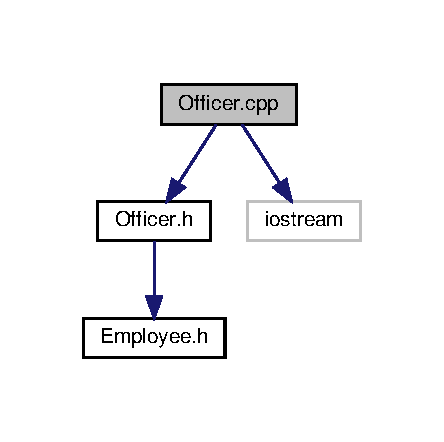
\includegraphics[width=213pt]{Officer_8cpp__incl}
\end{center}
\end{figure}


\subsection{Detailed Description}
\hyperlink{classOfficer}{Officer} class implementation. 

\begin{DoxyAuthor}{Author}
Ethan Buchanan 
\end{DoxyAuthor}
\begin{DoxyDate}{Date}
2022-\/11-\/15 \hyperlink{classOfficer}{Officer} class implementation with evilness 
\end{DoxyDate}

\hypertarget{Supervisor_8cpp}{}\section{Supervisor.\+cpp File Reference}
\label{Supervisor_8cpp}\index{Supervisor.\+cpp@{Supervisor.\+cpp}}


\hyperlink{classSupervisor}{Supervisor} implementatiom.  


{\ttfamily \#include \char`\"{}Supervisor.\+h\char`\"{}}\newline
{\ttfamily \#include $<$iostream$>$}\newline
Include dependency graph for Supervisor.\+cpp\+:\nopagebreak
\begin{figure}[H]
\begin{center}
\leavevmode
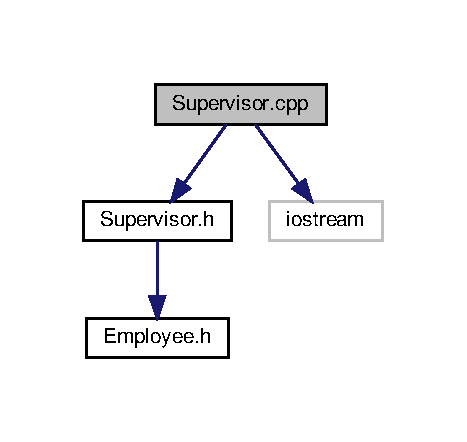
\includegraphics[width=224pt]{Supervisor_8cpp__incl}
\end{center}
\end{figure}


\subsection{Detailed Description}
\hyperlink{classSupervisor}{Supervisor} implementatiom. 

\begin{DoxyAuthor}{Author}
Ethan Buchanan 
\end{DoxyAuthor}
\begin{DoxyDate}{Date}
2022-\/11-\/15 \hyperlink{classSupervisor}{Supervisor} with extra supervised 
\end{DoxyDate}

\hypertarget{Supervisor_8h}{}\section{Supervisor.\+h File Reference}
\label{Supervisor_8h}\index{Supervisor.\+h@{Supervisor.\+h}}


\hyperlink{classSupervisor}{Supervisor} class implementation.  


{\ttfamily \#include \char`\"{}Employee.\+h\char`\"{}}\newline
Include dependency graph for Supervisor.\+h\+:\nopagebreak
\begin{figure}[H]
\begin{center}
\leavevmode
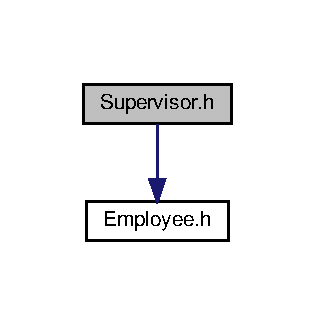
\includegraphics[width=151pt]{Supervisor_8h__incl}
\end{center}
\end{figure}
This graph shows which files directly or indirectly include this file\+:\nopagebreak
\begin{figure}[H]
\begin{center}
\leavevmode
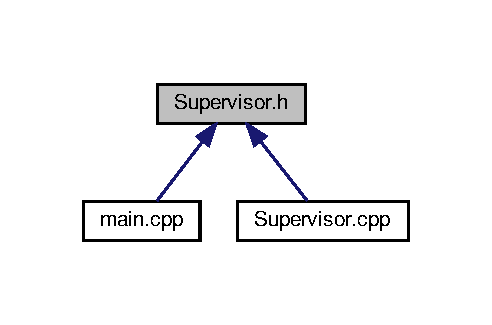
\includegraphics[width=236pt]{Supervisor_8h__dep__incl}
\end{center}
\end{figure}
\subsection*{Classes}
\begin{DoxyCompactItemize}
\item 
class \hyperlink{classSupervisor}{Supervisor}
\end{DoxyCompactItemize}


\subsection{Detailed Description}
\hyperlink{classSupervisor}{Supervisor} class implementation. 

\begin{DoxyAuthor}{Author}
Ethan Buchanan 
\end{DoxyAuthor}
\begin{DoxyDate}{Date}
2022-\/11-\/15 Derived from E\+Mployee class 
\end{DoxyDate}

%--- End generated contents ---

% Index
\backmatter
\newpage
\phantomsection
\clearemptydoublepage
\addcontentsline{toc}{chapter}{Index}
\printindex

\end{document}
